% Author: Izaak Neutelings (January 2021)
\documentclass[border=3pt,tikz]{standalone}
\usepackage{amsmath}
\usepackage{tikz}
\usepackage{physics}
\usepackage[outline]{contour} % glow around text
%\usetikzlibrary{intersections}
%\usetikzlibrary{decorations.markings}
\usetikzlibrary{angles,quotes} % for pic
\usetikzlibrary{bending} % for arrow head angle
\contourlength{1.0pt}
\usetikzlibrary{3d}

\tikzset{>=latex} % for LaTeX arrow head
\usepackage{xcolor}
\colorlet{myblue}{blue!65!black}
\colorlet{mydarkblue}{blue!50!black}
\colorlet{myred}{red!65!black}
\colorlet{mydarkred}{red!40!black}
\colorlet{veccol}{green!70!black}
\colorlet{vcol}{green!70!black}
\colorlet{xcol}{blue!85!black}
%\colorlet{projcol}{xcol!60}
%\colorlet{unitcol}{xcol!60!black!85}
%\colorlet{myred}{red!90!black}
%\colorlet{mypurple}{blue!50!red!80!black!80}
\tikzstyle{vector}=[->,very thick,xcol,line cap=round]
\tikzstyle{xline}=[myblue,very thick]
\tikzstyle{yzp}=[canvas is zy plane at x=0]
\tikzstyle{xzp}=[canvas is xz plane at y=0]
\tikzstyle{xyp}=[canvas is xy plane at z=0]
\def\tick#1#2{\draw[thick] (#1) ++ (#2:0.12) --++ (#2-180:0.24)}
\def\N{100}


\begin{document}


% COMPLEX
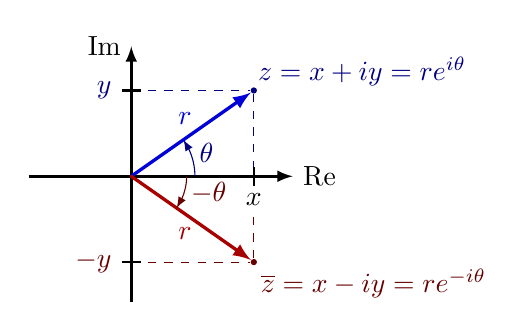
\begin{tikzpicture}
  \def\xmax{2.0}
  \def\ymax{1.6}
  \def\R{1.9}
  \def\ang{35}
  \coordinate (O) at (0,0);
  \coordinate (R) at (\ang:\R);
  \coordinate (-R) at (-\ang:\R);
  \coordinate (X) at ({\R*cos(\ang)},0);
  \coordinate (Y) at (0,{\R*sin(\ang)});
  \coordinate (-Y) at (0,{-\R*sin(\ang)});
  \node[fill=mydarkblue,circle,inner sep=0.8] (R') at (R) {};
  \node[fill=mydarkred,circle,inner sep=0.8] (-R') at (-R) {};
  \node[mydarkblue,above right=-2] at (R') {$z=x+iy=re^{i\theta}$};
  \node[mydarkred,below right=-1] at (-R') {$\overline{z}=x-iy=re^{-i\theta}$};
  \draw[dashed,mydarkblue]
    (Y) -- (R') --++ (0,{0.1-\R*sin(\ang)});
  \draw[dashed,mydarkred]
    (-Y) -- (-R') --++ (0,{\R*sin(\ang)-0.45});
  \draw[->,line width=0.9] (-0.65*\xmax,0) -- (\xmax+0.05,0) node[right] {Re};
  \draw[->,line width=0.9] (0,-\ymax) -- (0,\ymax+0.05) node[left] {Im};
  \draw[vector] (O) -- (R') node[pos=0.55,above left=-2] {$r$};
  \draw[vector,myred] (O) -- (-R') node[pos=0.55,below left=-2] {$r$};
  \draw pic[->,"$\theta$",mydarkblue,draw=mydarkblue,angle radius=23,angle eccentricity=1.24]
    {angle = X--O--R};
  \draw pic[<-,"$-\theta$"{right=-1},mydarkred,draw=mydarkred,angle radius=20,angle eccentricity=1]
    {angle = -R--O--X};
  %\tick{X}{90} node[scale=0.9,left=6,below right=-2] {$x = r\cos\theta$};
  \tick{X}{90} node[scale=1,below=-1] {$x$};
  \tick{Y}{ 0} node[mydarkblue,scale=1,left] {$y$}; %r\sin\theta = 
  \tick{-Y}{ 0} node[mydarkred,scale=1,left] {$-y$};
\end{tikzpicture}


% COMPLEX numbers
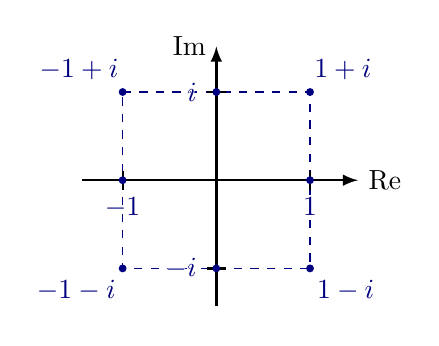
\begin{tikzpicture}
  \def\xmax{1.7}
  \def\ymax{1.6}
  \def\re{0.7*\xmax}
  \def\im{0.7*\ymax}
  \coordinate (O) at (0,0);
  \draw[dashed,mydarkblue]
    (-\re,\im) -| (\re,-\im) -| cycle;
  \draw[->,line width=0.9] (-\xmax,0) -- (\xmax+0.1,0) node[right] {Re};
  \draw[->,line width=0.9] (0,-\ymax) -- (0,\ymax+0.1) node[left] {Im};
  \tick{\re,0}{90} node[mydarkblue,scale=1,below=-1] {\contour{white}{$1$}};
  \tick{-\re,0}{90} node[mydarkblue,scale=1,below=-1] {\contour{white}{$-1$}};
  \tick{0,\im}{ 0} node[mydarkblue,scale=1,left] {\contour{white}{$i$}}; %r\sin\theta = 
  \tick{0,-\im}{ 0} node[mydarkblue,scale=1,left] {\contour{white}{$-i$}};
  \fill[mydarkblue]
    (   0, \im) circle(0.05)
    (   0,-\im) circle(0.05)
    ( \re,   0) circle(0.05)
    (-\re,  0) circle(0.05)
    ( \re, \im) circle(0.05)
      node[mydarkblue,scale=1,above right=-2] {\strut$1+i$}
    ( \re,-\im) circle(0.05)
      node[mydarkblue,scale=1,below right=-1] {\strut$1-i$}
    (-\re, \im) circle(0.05)
      node[mydarkblue,scale=1,above left=-2] {\strut$-1+i$}
    (-\re,-\im) circle(0.05)
      node[mydarkblue,scale=1,below left=-1] {\strut$-1-i$};
\end{tikzpicture}


% COMPLEX OSCILLATOR
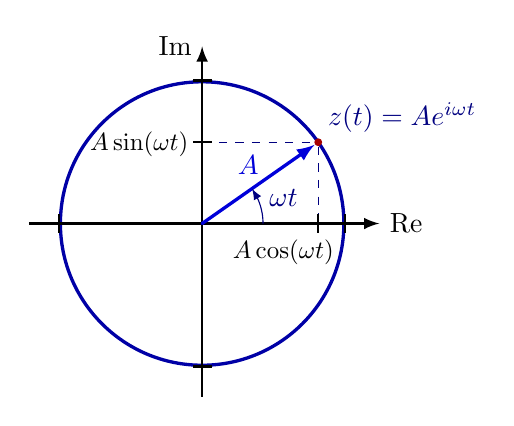
\begin{tikzpicture}
  \def\xmax{2.2}
  \def\ymax{2.2}
  \def\R{1.8}
  \def\ang{35}
  \coordinate (O) at (0,0);
  \coordinate (R) at (\ang:\R);
  \coordinate (X) at ({\R*cos(\ang)},0);
  \coordinate (Y) at (0,{\R*sin(\ang)});
  \draw[xline] (O) circle (\R); %0.995*\R
  \node[fill=myred,circle,inner sep=1] (R') at (R) {};
  \node[mydarkblue,above right=0] at (R') {$z(t)=Ae^{i\omega t}$};
  \draw[dashed,mydarkblue]
    (Y) -- (R') --++ (0,{0.1-\R*sin(\ang)});
  \draw[->,line width=0.9] (-\xmax,0) -- (\xmax+0.05,0) node[right] {Re};
  \draw[->,line width=0.9] (0,-\ymax) -- (0,\ymax+0.05) node[left] {Im};
  \draw[vector] (O) -- (R') node[pos=0.55,above left=-2] {$A$};
  \draw pic[->,"$\omega t$",mydarkblue,draw=mydarkblue,angle radius=22,angle eccentricity=1.4]
    {angle = X--O--R};
  \tick{0,\R+0.015}{0}; %node[scale=0.9,left=2] {\contour{white}{$R$}};
  \tick{\R+0.015,0}{90}; %node[scale=0.9,right=1,below=0] {\contour{white}{$R$}};
  \tick{0,-\R-0.015}{0};
  \tick{-\R-0.015,0}{90};
  \tick{X}{90} node[scale=0.9,left=14,below=-1] {$A\cos(\omega t)$}; %{\contour{white}{$A\cos(\omega t)$}};
  \tick{Y}{ 0} node[scale=0.9,below=1,left=-2] {$A\sin(\omega t)$}; % {\contour{white}{$A\sin(\omega t)$}};
\end{tikzpicture}


% COMPLEX OSCILLATOR 3D
\def\xang{-13}
\def\zang{45}
\begin{tikzpicture}[x=(\xang:0.9), y=(90:0.9), z=(\zang:1.1)]
  \message{^^JSynthesis 3D}
  \def\xmax{8.8}         % max x axis
  \def\ymin{-1.5}        % min y axis
  \def\ymax{1.6}         % max y axis
  \def\zmax{1.6}         % max z axis
  \def\xf{1.17*\xmax}    % x position frequency axis
  \def\A{(0.70*\ymax)}   % amplitude
  \def\T{(0.335*\xmax)}  % period
  \def\w{\zmax/11.2}     % spacing components
  \def\ang{47}           % angle
  \def\s{\ang/360*\T}    % time component
  \def\x{\A*cos(\ang)}   % real component
  \def\y{\A*sin(\ang)}   % imaginary component
  
  % COMPLEX PLANE
  \begin{scope}[shift={(-1.6*\zmax,0,0)}]
    \draw[black,fill=white,opacity=0.3,yzp]
      (-1.25*\zmax,-1.25*\ymax) rectangle (1.4*\zmax,1.25*\ymax);
    \draw[->,thick] (0,\ymin,0) -- (0,\ymax+0.02,0)
      node[pos=1,left=0,yzp] {Im};
    \draw[->,thick] (0,0,-\zmax) -- (0,0,\zmax+0.02)
      node[right=1,below=0,yzp] {Re} coordinate (X);
    %\node[scale=1,yzp] at (0,-\ymax,0) {Complex plane};
    \draw[xline,yzp] (0,0) circle(0.991*\A) coordinate (O);
    \fill[myred,yzp] (\ang:{\A}) circle(0.07) coordinate(P);
    \node[mydarkblue,above=3,right=-5,yzp,scale=0.8] at (P) {$z(t)=Ae^{i\omega t}$};
    \draw[vector,thick,yzp] (0,0) -- (\ang:{\A-0.03}) coordinate (R);
    \draw pic[-{>[flex'=1]},draw=mydarkblue,angle radius=14,angle eccentricity=1,
              "$\omega t$"{above=0,right=-0.5,yslant=0.69,scale=0.8},mydarkblue,yzp]
      {angle = X--O--R};
    \tick{0,0,{\A}}{90};
    \tick{0,0,{-\A}}{90};
    \tick{0,{\A},0}{\zang};
    \tick{0,{-\A},0}{\zang};
  \end{scope}
  
  % IMAGINARY
  \begin{scope}[shift={(0,0,1.9*\zmax)}]
    \draw[black,fill=white,opacity=0.3,xyp]
      (-0.5*\ymax,-1.2*\ymax) rectangle (1.10*\xmax,1.25*\ymax);
    \draw[->,thick] (-0.3*\ymax,0,0) -- (\xmax,0,0)
      node[below right=-2,xyp] {$t$ [s]};
    \draw[->,thick] (0,\ymin,0) -- (0,\ymax,0)
      node[left,xyp] {Im};
    \draw[xline,samples=\N,smooth,variable=\t,domain=-0.05*\T:0.95*\xmax]
      plot(\t,{\A*sin(360/\T*\t)},0);
    %\node[below=0,xyp] at (0.4*\xmax,-\ymax,0) {Imaginary component};
    \fill[myred,xyp] ({\s},{\y}) circle(0.07) coordinate(I);
    \draw[vector,thick,xyp] ({\s},0) --++ (0,{\y-0.03});
    \tick{0,{\A},0}{180};
    \tick{0,{-\A},0}{180};
    \tick{{\s},0,0}{90} node[right=0,below=-1,xyp] {$\omega t$};
    \tick{{\T},0,0}{90} node[right=0,below,xyp] {\contour{white}{$T$}};
    \tick{{2*\T},0,0}{90} node[right=0,below,xyp] {\contour{white}{$2T$}};
    \node[mydarkblue,below=0,xyp] at (0.4*\xmax,1.15*\ymax,0) {$y(t)=A\sin(\omega t)$};
  \end{scope}
  
  % REAL
  \begin{scope}[shift={(0,-1.8*\zmax,0)}]
    \draw[black,fill=white,opacity=0.3,xzp]
      (-0.5*\ymax,-1.4*\ymax) rectangle (1.10*\xmax,1.25*\ymax);
    \draw[->,thick] (-0.3*\ymax,0,0) -- (\xmax,0,0)
      node[below right=-1,xzp] {$t$ [s]};
    \draw[->,thick] (0,0,-\zmax) -- (0,0,\zmax)
      node[left=-1,xzp] {Re};
    \draw[xline,samples=\N,smooth,variable=\t,domain=-0.05*\T:0.95*\xmax]
      plot(\t,0,{\A*cos(360/\T*\t)});
    %\node[below=0,xzp] at (0.4*\xmax,-\ymax,0) {Real component};
    \fill[myred,xzp] ({\s},{\x}) circle(0.07) coordinate(R);
    \draw[vector,thick,xzp] ({\s},0) --++ (0,{\x-0.03});
    \tick{0,0,{\A}}{180};
    \tick{0,0,{-\A}}{180};
    \tick{{\s},0,0}{\zang} node[below=-1,xzp] {$\omega t$};
    \tick{{\T},0,0}{\zang} node[below,xzp] {$T$};
    \tick{{2*\T},0,0}{\zang} node[below,xzp] {$2T$};
    \node[mydarkblue,above=0,xzp] at (0.3*\xmax,-\ymax,0) {$x(t)=A\cos(\omega t)$};
  \end{scope}
  
  % COMPONENTS
  \draw[myred!80!black,dashed]
    (P) -- ({\s},{\y},{\x})
    (I) -- ({\s},{\y},{\x+0.05})
    ({\s},{\y-0.06},{\x}) -- (R);
  \draw[->,black,thick] (-0.1*\ymax,0,0) -- (\xmax,0,0) node[below right=-2] {$t$ [s]};
  \draw[->,black,thick] (0,\ymin,0,0) -- (0,\ymax+0.02,0) node[above] {Im};
  \draw[->,black,thick] (0,0,-\zmax) -- (0,0,\zmax+0.02) node[right=1,below=3] {Re};
  \foreach \i [evaluate={\tmin=max(-0.05*\T,(\i-0.05)*\T); \tmax=min(0.95*\xmax,(\i+1)*\T);}] in {0,...,2}{
    %\draw[white,line width=1.2] (\tmin,0,0) -- (\tmax,0,0);
    \draw[thick] (\tmin,0,0) -- (\tmax,0,0);
    \draw[xline,samples=0.4*\N,smooth,variable=\t]
      plot[domain=\tmin:\tmax](\t,{\A*sin(360/\T*\t)},{\A*cos(360/\T*\t)});
  }
  \draw[thick] (0,0,{0.9*\A}) -- (0,0,{\A});
  \fill[myred] ({\s},{\y},{\x}) circle(0.07) coordinate(Z);
  \draw[vector,thick] ({\s},0,0) --++ (0,{\y-0.03},{\x-0.03});
  \draw[xline,samples=0.3*\N,smooth,variable=\t,domain=\s+0.03:\s+0.4*\T,line cap=round]
    plot(\t,{\A*sin(360/\T*\t)},{\A*cos(360/\T*\t)});
  \tick{{\T},0,0}{90};
  \tick{{2*\T},0,0}{90};
  \tick{0,0,{\A}}{90};
  \tick{0,0,{-\A}}{90};
  \tick{0,{\A},0}{\zang};
  \tick{0,{-\A},0}{\zang};
  \draw[myred!80!black,dashed]
    ({\s},{\y-0.06},{\x}) --++ (0,-0.2*\ymax,0);
  
\end{tikzpicture}



% VECTOR ROTATION
\def\xmax{2.7}
\def\ymax{2.7}
\def\R{2.3}
\def\ang{28}
\def\dang{35}
\begin{tikzpicture}
  \coordinate (O) at (0,0);
  \coordinate (R) at (\ang:\R);
  \coordinate (Q) at (\ang+\dang:\R);
  \coordinate (X) at ({\R*cos(\ang)},0);
  \coordinate (Y) at (0,{\R*sin(\ang)});
  \coordinate (X') at ({\R*cos(\ang+\dang)},0);
  \coordinate (Y') at (0,{\R*sin(\ang+\dang)});
  %\draw[myblue] (O) circle (0.995*\R);
  \draw[myblue] (-10:\R) arc (-10:100:\R);
  \node[fill=myred,circle,inner sep=0.8] at (R) {};
  \node[fill=myred,circle,inner sep=0.8] at (Q) {};
  \node[mydarkblue,above right=-2] at (R) {$\vb{r}=(x,y)$};
  \node[mydarkblue,above right=-2] at (Q) {$\vb{r}'=(x',y')$};
  \draw[dashed,mydarkblue]
    (Y) -- (R) --++ (0,{0.1-\R*sin(\ang)});
  \draw[dashed,mydarkblue]
    (Y') -- (Q) --++ (0,{0.1-\R*sin(\ang+\dang)});
  \draw[->,line width=0.9] (-0.1*\xmax,0) -- (\xmax+0.05,0) node[right] {$x$};
  \draw[->,line width=0.9] (0,-0.1*\ymax) -- (0,\ymax+0.05) node[left] {$y$};
  \draw[vector] (O) -- (R);
  \draw[vector] (O) -- (Q);
  \draw pic[->,"$\phi$",mydarkblue,draw=mydarkblue,angle radius=20,angle eccentricity=1.35]
    {angle = R--O--Q};
  \tick{0,\R+0.015}{0};
  \tick{\R+0.015,0}{90};
  \tick{X}{90} node[scale=0.9,left=14,below=-1] {$x$};
  \tick{Y}{ 0} node[scale=0.9,below=1,left=-2] {$y$};
  \tick{X'}{90} node[scale=0.9,left=14,below=-1] {$x'$};
  \tick{Y'}{ 0} node[scale=0.9,below=1,left=-2] {$y'$};
\end{tikzpicture}


% COMPLEX ROTATION
\begin{tikzpicture}
  \coordinate (O) at (0,0);
  \coordinate (R) at (\ang:\R);
  \coordinate (Q) at (\ang+\dang:\R);
  \coordinate (X) at ({\R*cos(\ang)},0);
  \coordinate (Y) at (0,{\R*sin(\ang)});
  %\draw[myblue] (O) circle (0.995*\R);
  \draw[myblue] (-10:\R) arc (-10:100:\R);
  \node[fill=myred,circle,inner sep=0.8] at (R) {};
  \node[fill=myred,circle,inner sep=0.8] at (Q) {};
  \node[mydarkblue,above right=0] at (R) {$z=re^{i\theta}$};
  \node[mydarkblue,left=2,above right=0] at (Q) {$ze^{i\phi}=re^{i(\theta+\phi)}$};
  \draw[dashed,mydarkblue]
    (Y) -- (R) --++ (0,{0.1-\R*sin(\ang)});
  \draw[->,line width=0.9] (-0.1*\xmax,0) -- (\xmax+0.05,0) node[right] {Re};
  \draw[->,line width=0.9] (0,-0.1*\ymax) -- (0,\ymax+0.05) node[left] {Im};
  \draw[vector] (O) -- (R) node[pos=0.65,above left=-3] {$r$};
  \draw[vector] (O) -- (Q) node[pos=0.65,above left=-3] {$r$};
  \draw pic[->,"$\theta$",mydarkblue,draw=mydarkblue,angle radius=24,angle eccentricity=1.25]
    {angle = X--O--R};
  \draw pic[->,"$\phi$",mydarkblue,draw=mydarkblue,angle radius=20,angle eccentricity=1.35]
    {angle = R--O--Q};
  \tick{0,\R+0.015}{0};
  \tick{\R+0.015,0}{90};
  \tick{X}{90} node[scale=0.9,left=14,below=-1] {$r\cos\theta$};
  \tick{Y}{ 0} node[scale=0.9,below=1,left=-2] {$r\sin\theta$};
\end{tikzpicture}


\end{document}